\chapter{Wstęp}

\section{Przedstawienie problemu}

Problem, który rozważam to lokalizowanie zmian nowotworowych na zdjęciach wykonanych metodą rezonansu magnetycznego (MRI, ang. magnetic resonance imaging). Można podejść do niego od strony nadzorowanej, czyli bazować na danych przeanalizowanych wcześniej przez specjalistów, gdzie każdy przypadek został ręcznie obejrzany i oznaczony. O ile taka metoda ma wiele zalet, jak chociażby korzystanie z rzeczywistej wiedzy eksperckiej, to wykorzystywany zbiór jest bardzo kosztowny w przygotowaniu i dalszym rozwoju, a ponadto może być ograniczony jedynie do pojedynczej partii ciała. Zauważając te wady oraz łącząc je z obserwacją, że zmiany patologiczne tak na prawdę są rzadkie i są pewnym odstępstwem od normy, chce spróbować skorzystać z metody nienadzorowanej, w której to model nauczyłby się oszacowywać prawdopodobieństwo występowania pojedynczej próbki w pewnym kontekście. Przy takim podejściu mogę oznaczać obserwacje mało prawdopodobne jako właśnie te nowotworowe. Dodatkowo sama tak informacja może również pomóc specjalistom przy wyłanianiu obszarów podejrzanych. Model, na którego wykorzystanie się zdecydowałem to autoenkoder wariacyjny (VAE, ang. Variational Autoencoder), łączący sztuczne sieci neuronowe z modelowaniem probabilistycznym. Pomysł ten przetestuje początkowo na danych syntetycznych z wykorzystaniem zbioru MNIST.

\section{Sztuczne sieci neuronowe}

Sztuczne sieci neuronowe mają obecnie bardzo mocno ugruntowaną pozycję szczególnie w dziedzinie problemów związanych z analizą i przetwarzaniem obrazów. Pomimo, iż nie jest to nowy pomysł, dopiero ostatni wzrost w wydajności komputerów pozwolił na ich praktyczne zastosowanie. Z matematycznego punktu widzenia są to sparametryzowane nieliniowe funkcje o pewnej ustalonej strukturze. Składają się z prostych elementów zwanych neuronami, a one natomiast są pogrupowane w warstwy. Połączenia między warstwami definiują przepływ danych. 'Nauka' sieci neuronowych polega na optymalizacji pewnej funkcji straty, czyli wyznaczeniu takich parametrów, żeby osiągnąć minimalny koszt. Do tego celu często korzysta się z metod opartych na Stochastic Gradient Descent, a przy wybranej strukturze można w efektywny sposób zastosować algorytm propagacji wstecznej. W dalszej części pracy będę używał prostszej nazwy - sieci neuronowe. Przykładowa architektura sieci neuronowych jest zaprezentowana na rysunku \ref{fig:neural_nets}.

\begin{figure}[h!]
    \centering
    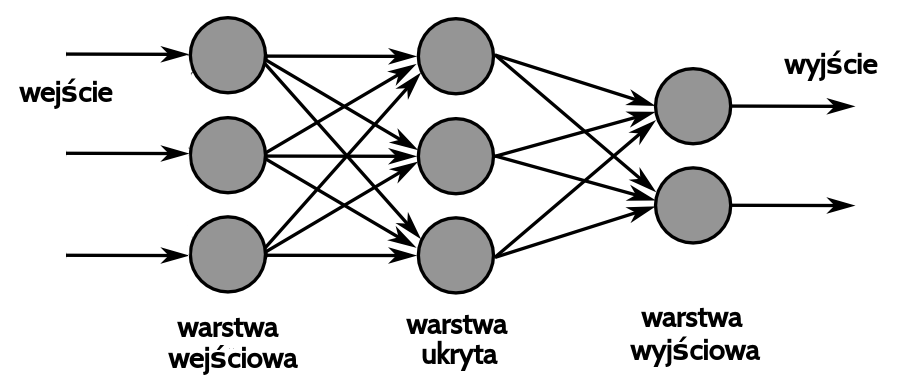
\includegraphics[width=0.6\textwidth]{images/neural_nets}
    \caption{Przykładowy model sieci neuronowej}
    \label{fig:neural_nets}
\end{figure}

\section{Uczenie nadzorowane i bez nadzoru}

Są to dwa różne rodzaje problemów z dziedziny uczenia maszynowego. W przypadku uczenia nadzorowanego wiemy jaką chcemy uzyskać odpowiedź dla danego wejścia i próbujemy tak dobrać parametry modelu, żeby odpowiadał on z jak największą poprawnością. Przykładowymi zadaniami tego rodzaju są regresja oraz klasyfikacja, która nawiasem mówiąc może zostać uznana za problem regresji, ale na dyskretnym, skończonym zbiorze.

Inaczej jest w sytuacji bez nadzoru. Tam dla danych wejściowych nie znamy interesującej nas odpowiedzi i staramy się tak zbudować model, żeby był on w stanie sam ją wydobyć. Zazwyczaj interesuje nas rozwiązanie takich problemów jak estymacja rozkładu prawdopodobieństwa z którego pochodzą dane, klasteryzacja, redukcja wymiarowości czy wydajne kodowanie danych. Jednym z modeli wykorzystywanym w tej klasie zadań jest właśnie autoenkoder.

W przypadku identyfikacji próbek odstających można zwracać uwagę na ich estymowane prawdopodobieństwo oraz efektywność kodowania i dekodowania, które oba powinny być niskie.

\section{Autoenkoder}

Jest to jeden z rodzai sieci neuronowych, służący do znajdowania wydajnej reprezentacji danych, co jak wspomniałem wcześniej jest przykładem nauki bez nadzoru. Myślę, że mogę go określić mianem nieliniowej alternatywy dla klasycznej statystycznej metody analizy głównych składowych (PCA, ang. principal component analysis). W autoenkoderach można wyróżnić dwie połączone ze sobą części zwane enkoderem i dekoderem. Zadaniem enkodera jest wyprodukowanie właśnie tej reprezentacji, podczas gdy dekoder służy do odtworzenia z niej oryginalnej postaci. Zależy nam na tym, żeby wyjście było w jakimś sensie jak najbardziej podobne do wejścia przy zachowaniu odpowiednio małej wymiarowości kodowania. Jest to pewnego rodzaju balansowanie pomiędzy ilością informacji, na których przepływ się zgadzamy, a ich jakością. W szczególności można pomyśleć o takiej patologicznej sytuacji jak ustalenie rozmiaru reprezentacji równej rozmiarowi danych wejściowych, co prawdopodobnie będzie skutkować idealnymi rekonstrukcjami, ale przy okazji zerową wiedzą płynącą z takiego modelu. Analogicznie można rozważyć przypadek kiedy obszar kodowania jest za mały. Model w takiej sytuacji skupi się jedynie na przekazaniu wyłącznie trywialnych cech, żeby mimo wszystko jakkolwiek odtworzyć dane. Poglądowy schemat budowy znajduje się na rysunku \ref{fig:autoenc}.

\begin{figure}[h!]
    \centering
    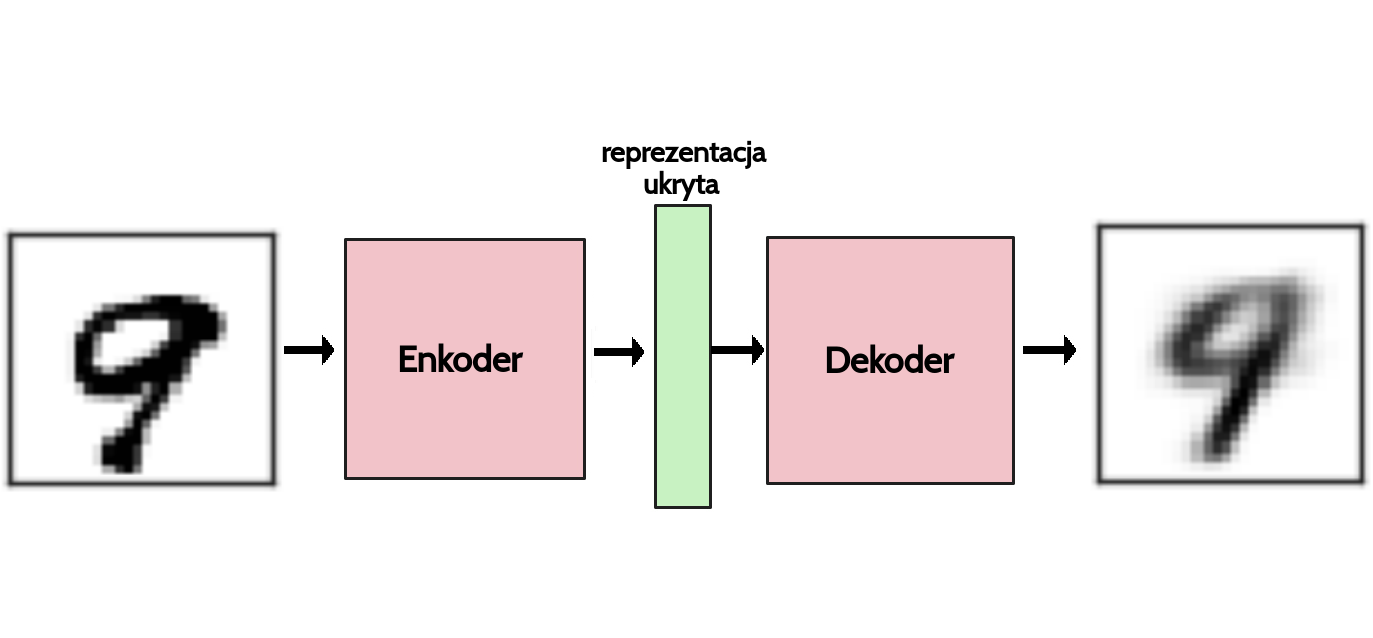
\includegraphics[width=1\textwidth]{images/autoenc}
    \caption{Architektura autoenkodera}
    \label{fig:autoenc}
\end{figure}

W przypadku obrazów na funkcję straty często wybierany jest błąd średniokwadratowy (MSE, ang. Mean Squared Error).

\begin{equation}
\mathrm { MSE } = \frac { 1 } { n } \sum _ { i = 1 } ^ { n } \left( Y _ { i } - \hat { Y } _ { i } \right) ^ { 2 }
\end{equation}
gdzie:
\begin{conditions}
    Y_i             &  oryginalne dane \\
    \hat{Y}_{i}     &  zrekonstruowane dane
\end{conditions}

Wymagającym sprostowania może być fakt, iż mimo mówimy jakie oczekujemy wyjście z modelu, w sensie rekonstrukcji, to dalej jest to problem typu nauki bez nadzoru, ponieważ rzeczywistą szukaną przez nas wiedzą jest umiejętność kodowania danych i osobno ich dekodowania. Chciałbym w tym miejscu zastanowić się co dzięki temu zyskujemy. Już teraz zaletą jest oczywiście redukcja wymiarowości, która ułatwia późniejszą analizę danych oraz pozwala na ich kompresję i ewentualne odszumianie. Dodatkowo wydaje się, że mając wytrenowany dekoder, na konkretnej rodzinie danych, moglibyśmy zaaplikować do niego jakieś nowe kodowanie i otrzymać w ten sposób wynik pochodzący z oryginalnej dziedziny, czyli wykorzystać go jako generator nowych próbek. Niestety ten pomysł ma taki problem, że podczas nauki nie ma żadnej kontroli nad tym jak dane zostaną rozmieszczone w przestrzeni, która notabene jest nieskończona (z ograniczeniem do pojemności liczb zmiennoprzecinkowych). W takim razie nie wiemy jaka podprzestrzeń odpowiada tym kodowaniom, które są sensownie dekodowane. Jest to potrzebne przy generowaniu. Dodatkowo jeśli przestrzeń byłaby nieciągła, to niemożliwe byłoby interpolowanie pomiędzy próbkami. Znaczącym problemem jest natomiast to, że kodowanie jako wektor liczb jest bardzo precyzyjną informacją, co może doprowadzić do przeuczenia modelu i błędnego działania na danych pochodzących z poza zbioru treningowego.

\section{Autoenkoder wariacyjny} \label{sec:vae}

Autoenkoder wariacyjny (VAE, ang. Variational Autoencoder) rozszerza założenia podstawowej architektury o wprowadzenie modelowania rozkładu prawdopodobieństwa dla reprezentacji ukrytej. W odróżnieniu od podstawowej wersji enkoder nie produkuje pojedynczego wektora, ale dwa wektory interpretowane odpowiednio jako średnie $\mu$ oraz wariancje $\sigma$ dla rozkładu Gaussa. Dopiero na podstawie tych parametrów formowane jest kodowanie, gdzie $i$-ta wartość losowana jest z $\mathcal{N}(\mu_{i},\,\sigma_{i}^{2})$, które aplikowane zostaje do dekodera i rekonstruowana jest na podstawie niego pierwotna próbka. Takie podejście znaczy, że nawet dla tego samego wejścia i podczas gdy średnie oraz odchylenia pozostaną niezmienne, to i tak reprezentacja będzie się różnić właśnie ze względu na występującą losowość. Zmodyfikowany schemat został przedstawiony na rysunku \ref{fig:vae_model}.

\begin{figure}[h!]
    \centering
    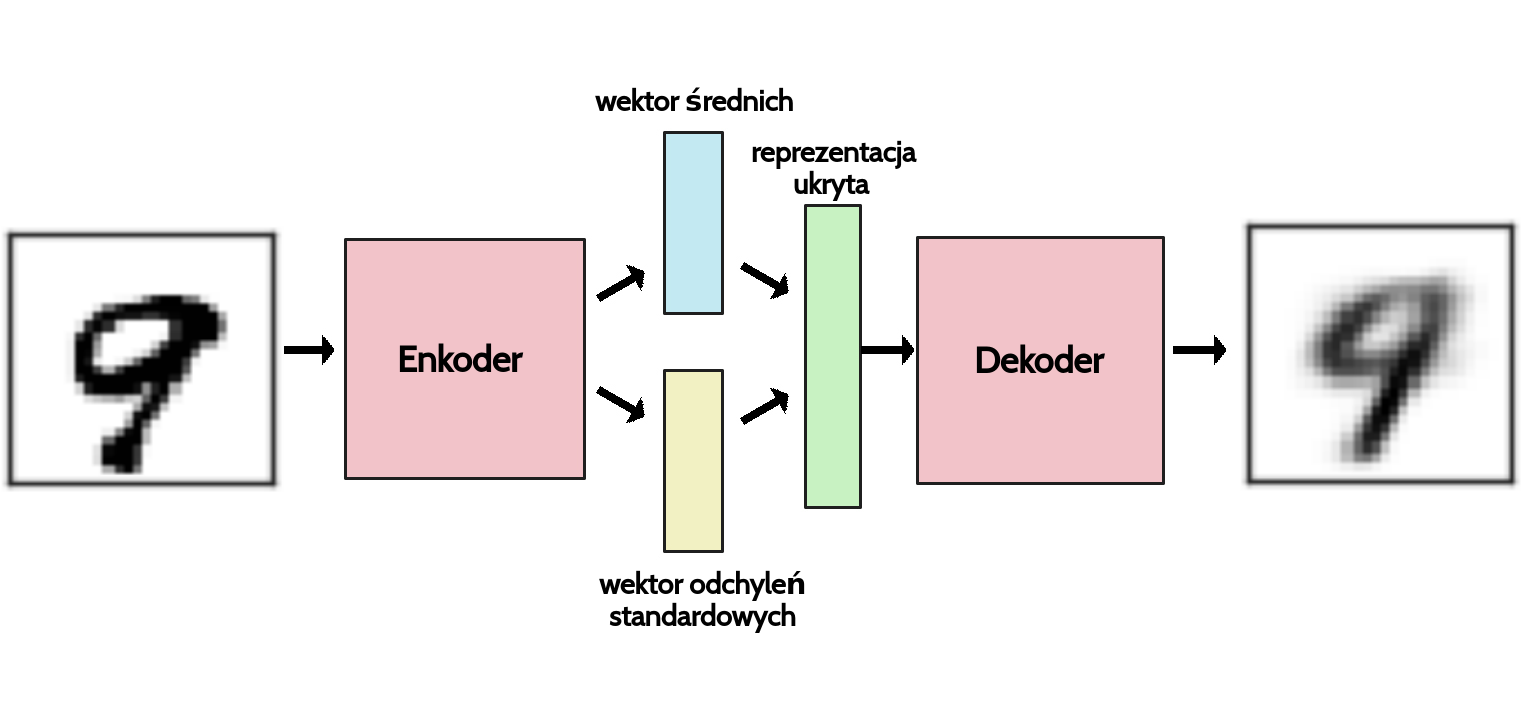
\includegraphics[width=1.0\textwidth]{images/vae}
    \caption{Architektura autoenkodera wariacyjnego}
    \label{fig:vae_model}
\end{figure}

Intuicyjnie wektor średnich oznacza miejsce, gdzie zakodowana zmienna powinna być wycentrowana, natomiast odchylenie kontroluje obszar, wokół którego kodowanie może się różnić. Sytuację tę zaprezentowałem na wykresie \ref{fig:vae_vs_stand}, przy czym porównałem z podstawową wersją. W jej przypadku informacja wychodząca z enkodera jest bardzo precyzyjna, natomiast w obecnie rozważanym modelu, dzięki dodaniu szumu, zostaje ona rozmyta. Taki zabieg ma za zadanie ograniczyć zjawisko przeuczenia oraz wprowadzić pewną lokalną ciągłość w przestrzeni. Jest to wynikiem tego, że gdy kodowanie losowane jest z wnętrza kuli, notabene o nieskończonym promieniu, ale ustalonej gęstości, to dekoder zmuszony jest nauczyć się, że nie tylko pojedynczy punkt odnosi się do danej próbki, ale i również jego całe lokalne sąsiedztwo. To pozwala dekodować nie tylko specyficzne reprezentacje (pozostawiając przestrzeń nieciągłą), ale też te trochę różniące się, ponieważ model narażony jest na szereg zmian kodowania tego samego wejścia podczas treningu.

\begin{figure}[h!]
  \centering
  \begin{subfigure}[b]{0.4\linewidth}
    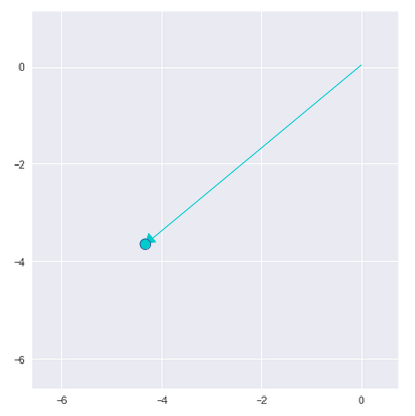
\includegraphics[width=1.0\textwidth]{images/vae_vs_stand_a}
    \caption{Standardowy autoenkoder}
  \end{subfigure}
  \begin{subfigure}[b]{0.4\linewidth}
    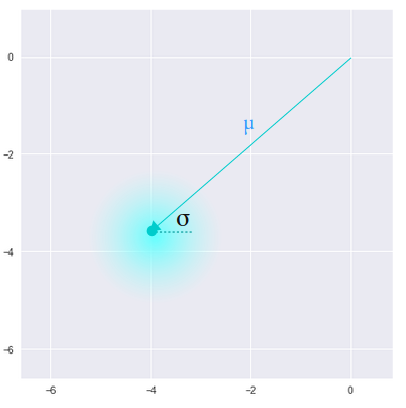
\includegraphics[width=1.0\textwidth]{images/vae_vs_stand_b}
    \caption{Autoenkoder wariacyjny}
  \end{subfigure}
  \caption{Porównanie precyzji informacji dostarczanych przez enkodery}
  \label{fig:vae_vs_stand}
\end{figure}

Model jest teraz wystawiony na pewien stopień lokalnej zmienności przez wprowadzenie szumu do kodowania pojedynczej próbki, co skutkuje ciągłą przestrzenią w reprezentacji ukrytej dla lokalnego sąsiedztwa. Jednak na razie nie ma ograniczeń co do wartości jakie mogą być przyjmowane przez wektory $\mu$ i $\sigma$, a w rezultacie enkoder może nauczyć się generować bardzo różne $\mu$ dla różnych klas i grupować je minimalizując $\sigma$, upewniając się przy tym, że samo kodowanie nie różni się zbytnio dla tej samej próbki. W szczególności prawdopodobnym jest wystąpienie tak patologicznej sytuacji, gdzie $\sigma$ zawsze wynosi 0, przez co nowy model nie będzie różnić się w działaniu od jego podstawowej wersji, włącznie z uwzględnieniem wad, które starał się wyeliminować. Omawiany przeze mnie przykład przedstawiony jest na rysunku \ref{fig:vae_nolimits}. Oczekiwaną sytuacją byłoby rozłożenie danych blisko siebie, ale z zachowaniem ich separowalności. Pozwoliłoby to na gładką interpolacje pomiędzy próbkami i generowanie nowych danych.

\begin{figure}[h!]
  \centering
  \begin{subfigure}[b]{0.4\linewidth}
    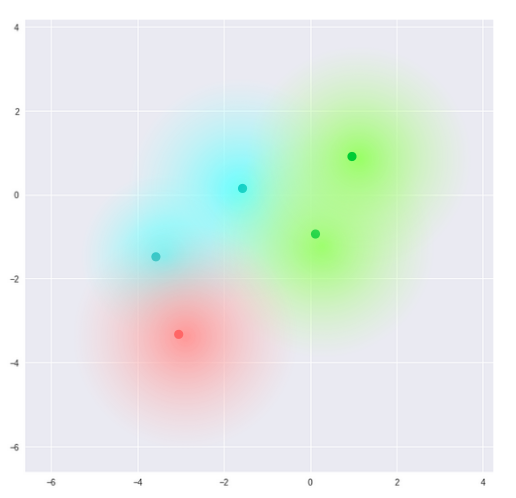
\includegraphics[width=1.0\textwidth]{images/vae_nolimits_a}
    \caption{Oczekiwany układ}
  \end{subfigure}
  \begin{subfigure}[b]{0.4\linewidth}
    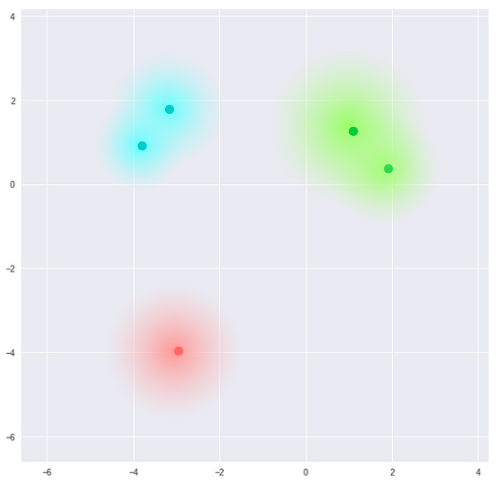
\includegraphics[width=1.0\textwidth]{images/vae_nolimits_b}
    \caption{Niezamierzony układ}
  \end{subfigure}
  \caption{Porównanie rozkładów danych ze względu na brak ograniczeń dla reprezentacji. Przy czym ten pierwszy jest lepszy ponieważ obszar z którego generować można nowe dane jest spójny}
  \label{fig:vae_nolimits}
\end{figure}

W celu osiągnięcia zamierzonych rezultatów, należy wzbogacić funkcję straty o koszt dywergencji Kullbacka-Leiblera, która mierzy różnicę pomiędzy dwoma rozkładami prawdopodobieństwa. Minimalizowanie go oznacza optymalizowanie parametrów rozkładu ($\mu$ i $\sigma$), tak żeby jak najbardziej przypominał docelowy rozkład, który w przypadku autoenkodera wariacyjnego będzie standardowym rozkładem normalnym ($\mu = 0$,  $\sigma = 1$).
Przy takim wyborze dane powinny zostać rozrzucone dookoła $\vec{0}$ i nie pozostawiać pustych miejsc w przestrzeni ukrytej.

\begin{equation}
\mathrm { KLD } = \sum _ { i = 1 } ^ { n } \sigma _ { i } ^ { 2 } + \mu _ { i } ^ { 2 } - \log \left( \sigma _ { i } \right) - 1
\end{equation}


\subsection{Model probabilistyczny}

To co do tej pory napisałem odnośnie autoenkodera wariacyjnego raczej trzeba uznać za zbiór intuicji i oczekiwań. W tym rozdziale chciałbym pokazać jego funkcjonowanie od strony probabilistycznej.

Myślimy, że autoenkoder wariacyjny modeluje wspólny rozkład prawdopodobieństwa $p(x, z)$, gdzie $x$ to obserwowane dane, a $z$ to zmienna ukryta. Możemy to rozpisać w następujący sposób $p(x, z) = p(x|z)p(z)$. Wróćmy teraz do założeń, gdzie zależało nam na produkowaniu dobrych reprezentacji dla określonej próbki, czyli wyznaczeniu prawdopodobieństwa a posteriori $p(z|x)$. Zgodnie z twierdzeniem Bayesa
$$p(z|x)=\frac{p(x|z)p(z)}{p(x)}$$

Problem jest jednak z mianownikiem $p(x)$. Można go obliczyć marginalizując zmienne ukryte, ale wtedy $p(x)=\int{p(x|z)p(z)dz}$ i wymaga to przejrzenia wszystkich kombinacji reprezentacji ukrytych. W takim razie w jakiś inny sposób trzeba policzyć to prawdopodobieństwo $p(z|x)$.

Korzystając z wnioskowania wariacyjnego (ang. variational inference) przybliżymy tę wartość na podstawie rodziny rozkładów $q _ { \lambda } ( z | x )$, gdzie jeśli $q$ byłoby rozkładem Gaussa to $\lambda _ { x _ { i } } = \left( \mu _ { x _ { i } } , \sigma _ { x _ { i } } ^ { 2 } \right)$

Do sprawdzenia jak dobrze przybliżamy te rozkłady możemy skorzystać z dywergencji Kullbacka-Leiblera, która mierzy ilość straconych informacji, kiedy używamy $q$ do zaokrąglenia $p$ (w natach)

\begin{equation}
\begin{split}
\mathbb { K } \mathbb { L } \left( q _ { \lambda } ( z | x ) \| p ( z | x ) \right) =
\mathbf { E } _ { q } \left[ \log \frac{q _ { \lambda } ( z | x )}{p ( z | x )} \right] = \\
\mathbf { E } _ { q } \left[ \log p ( z | x ) \right] - \mathbf { E } _ { q } \left[ \log \frac{q _ { \lambda } ( x, z )}{p ( x )} \right] = \\
\mathbf { E } _ { q } \left[ \log q _ { \lambda } ( z | x ) \right] - \mathbf { E } _ { q } [ \log p ( x , z ) ] + \log p ( x )
\end{split}
\end{equation}

Celem jest znalezienie parametru $\lambda$, który minimalizuje tę sumę.

\begin{equation}
q _ { \lambda } ^ { * } ( z | x ) = \arg \min _ { \lambda } \mathbb { K } \mathbb { L } \left( q _ { \lambda } ( z | x ) \| p ( z | x ) \right)
\end{equation}

Niestety nie jest to obliczalne ze względu an ponownie występujący element $p(x)$, tak jak w dyskusji powyżej. Możemy jednak rozważyć funkcję 

\begin{equation}
E L B O ( \lambda ) = \mathbf { E } _ { q } [ \log p ( x , z ) ] - \mathbf { E } _ { q } \left[ \log q _ { \lambda } ( z | x ) \right]
\end{equation}

Zauważmy, że łączy się to z powyższą równością co przepiszmy jako

\begin{equation}
\log p ( x ) = E L B O ( \lambda ) + \mathbb { K } \mathbb { L } \left( q _ { \lambda } ( z | x ) \| p ( z | x ) \right)
\end{equation}

Skorzystajmy teraz z faktu, że dywergencja Kullbacka-Leiblera jest nieujemna, czyli zamiast ją minimalizować możemy maksymalizować $ELBO$. Wniosek jest taki, że $ELBO$ pozwala oszacowywać dolne prawdopodobieństwo na wystąpienie danej próbki, a dodatkowo jest to wartość obliczalna.

Przy założeniu, że dane są niezależne, które wykonujemy w przypadku autoenkodera, możemy rozłożyć $ELBO$ na sumę składników, gdzie każdy dotyczy tylko pojedynczej próbki. Wtedy dla pojedynczego elementu otrzymujemy

\begin{equation}
\begin{split}
E L B O _ { i } ( \lambda ) = \mathbf { E } _ { q } [ \log p ( x_i , z ) ] - \mathbf { E } _ { q } \left[ \log q _ { \lambda } ( z | x_i ) \right] = \\
\mathbf { E } _ { q } [ \log p ( x_i | z ) p(z){} ] - \mathbf { E } _ { q } \left[ \log q _ { \lambda } ( z | x_i ) \right] = \\
\mathbf { E } _ { q } [ \log p ( x_i | z ){} ] + \mathbf { E } _ { q } [ \log p(z){} ] - \mathbf { E } _ { q } \left[ \log q _ { \lambda } ( z | x_i ) \right] = \\
\mathbf { E } _ { q } [ \log p ( x_i | z ){} ] - (\mathbf { E } _ { q } \left[ \log q _ { \lambda } ( z | x_i ) \right] - \mathbf { E } _ { q } [ \log p(z){} ])= \\
\mathbf { E } _ { q } [ \log p ( x_i | z ){} ] - \mathbb { K } \mathbb { L } \left( q _ { \lambda } ( z | x _ { i } ) \| p ( z ) \right) = \\
\mathbb { E } q _ { \lambda } ( z | x _ { i } ) \left[ \log p \left( x _ { i } | z \right) \right] - \mathbb { K } \mathbb { L } \left( q _ { \lambda } ( z | x _ { i } ) \| p ( z ) \right)
\end{split}
\end{equation}

Teraz już możemy połączyć to z sieciami neuronowymi. Do znalezienia parametrów dla $q _ { \theta } ( z | x , \lambda )$ posłuży enkoder, który z $x$ produkuje $\lambda$. Natomiast dekoder bierze reprezentację ukrytą i zwraca parametry dla rozkładu danych $p _ { \phi } ( x | z )$. Wartości $\theta$ i $\phi$ możemy też traktować jako parametry dla sieci neuronowej. Wtedy funkcja straty, którą będziemy minimalizować prezentuje się następująco

\begin{equation}
l _ { i } ( \theta , \phi ) = -E L B O _ { i } ( \theta , \phi ) = -\mathbb { E } q _ { \theta } ( z | x _ { i } ) \left[ \log p _ { \phi } \left( x _ { i } | z \right) \right] + \mathbb { K } \mathbb { L } \left( q _ { \theta } ( z | x _ { i } ) \| p ( z ) \right)
\end{equation}

Interpretacja:
\begin{itemize}[]
\item $-\mathbb { E } q _ { \theta } ( z | x _ { i } ) \left[ \log p _ { \phi } \left( x _ { i } | z \right) \right]$ można utożsamiać z błędem rekonstrukcji, gdyż odpowiada temu składnik $\log p(x|z)$, a w trakcie treningu ta liczb powinna być jak najmniejsza. Dodatkowo jest to potęgowane przez $q(z|x)$, czyli pewność co do reprezentacji ukrytej.

\item $\mathbb { K } \mathbb { L } \left( q _ { \theta } ( z | x _ { i } ) \| p ( z ) \right)$ można interpretować jako ilość przesyłanych informacji, ponieważ jeżeli model będzie chciał odejść od rozkładu a priori $p(z)$ to zapłaci za to karę, ale będzie w stanie przekazać wiadomość.
\end{itemize}

\section{Ocena jakości modelu}

\subsection{Krzywa ROC i AUC}

Krzywa ROC (Receiver Operating Characteristic) jest narzędziem do oceny poprawności klasyfikatora binarnego. Bazuje ona na wyliczaniu charakterystyki jakościowej modelu predykcji w wielu różnych punktach odcięcia. Działa to na takiej zasadzie, że model dla próbek przewiduje z jaką pewnością pochodzą z klasy 1. Następnie badane są różne progi i klasyfikowane przy ich użyciu obiekty. Dla uzyskanych klasyfikacji liczymy odsetek prawdziwych pozytywnych (TPR) oraz odsetek fałszywych pozytywnych (FPR) i nanosimy te wartości na wykres. Warto zauważyć, że dla losowego modelu jego wykres to prosta przechodząca przez (0, 0) i (1, 1). Dzieje się tak, ponieważ dla każdego progu połowa klasyfikacji będzie nad i połowa pod. Idealny model znajduje się w punkcie (0, 1).

Przydatne jest również obliczenie pola powierzchni pod krzywą AUROC (ang. Area Under the ROC). Pozwala ona ocenić ogólną skuteczność modelu bez wyboru konkretnego progu. Interpretuje się ją jako prawdopodobieństwo, że badany model predykcyjny oceni wyżej losowy element klasy pozytywnej od losowego elementu klasy negatywnej.
